\section{Proposed solutions}

\begin{frame}{Multivariate outlier detection}

    Two \textbf{methods} are presented, both \textbf{based on the concept of multivariate outlier detection in the frequency domain}:

    \begin{itemize}
        \item Mahalanobis Squared Distance (MSD)
        \item Principal Component Analysis (PCA)
    \end{itemize}

\end{frame}



\subsection{Mahalanobis Squared Distance (MSD)}

\begin{frame}{Mahalanobis Squared Distance (MSD) approach}

    The Mahalanobis Squared Distance (MSD) is a measure of the distance between a point and a distribution.


    \begin{columns}[c, onlytextwidth]

        \begin{column}{0.5\textwidth}

            It's defined as:
            \begin{equation}
                D_{MSD}^2 = (\mathbf{x} - \mathbf{\mu})^T \mathbf{\Sigma}^{-1} (\mathbf{x} - \mathbf{\mu})
            \end{equation}

            Where:
            \begin{itemize}
                \item $\mathbf{x}_{(m \times 1)}$ is the vector of the observations
                \item $\mathbf{\mu}_{(m \times 1)}$ is the mean of the observations
                \item $\mathbf{\Sigma}_{(m \times m)}$ is the covariance matrix of the observations
            \end{itemize}

        \end{column}

        \hfill

        \begin{column}{0.45\textwidth}

            \begin{figure}[H]
                \centering
                % https://it.mathworks.com/help/stats/mahal.html
                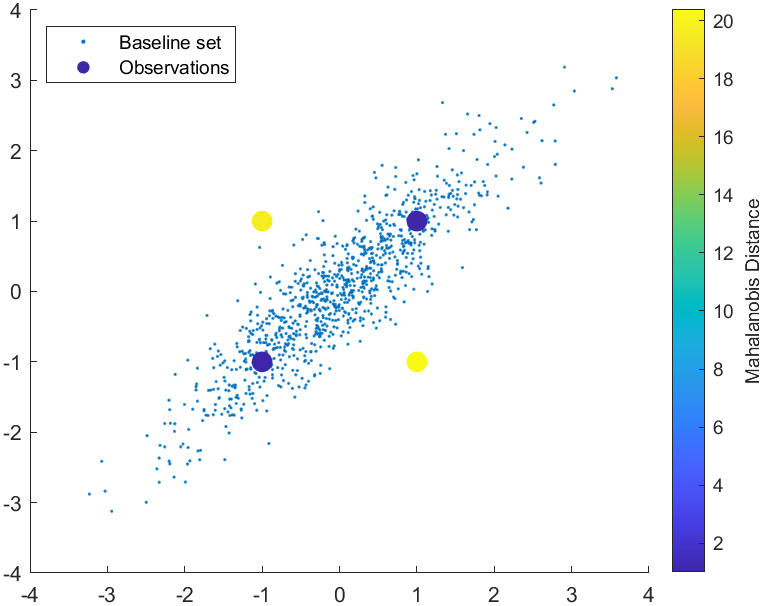
\includegraphics[width=\textwidth]{img/Mahalanobis-cloud-plot.png}
                \caption{Application example of the MSD index. \textcolor[HTML]{F5EC22}{Outliers} are clearly visible. Credit to: \textit{MathWorks}.}
            \end{figure}

        \end{column}

    \end{columns}

    \vspace{9pt}

    The MSD is used to detect outliers in the data, by computing the distance between observations and the distribution of the data.

\end{frame}



\begin{frame}{Issues of the MSD approach related to SHM}

    The MSD approach is \textbf{based on the assumption that the baseline data contains all the possible variations due to environmental effects} (e.g. temperature, vibrations noise, etc.).

    \vspace{9pt}

    To be effective then, the baseline data should be collected in a wide range of environmental conditions in order to capture all the possible variations, \textbf{which imply a long and expensive data collection campaign} that is not always feasible.

\end{frame}



\subsection{Principal Components Analysis (PCA)}

\begin{frame}{Principal Components Analysis (PCA) approach}

    The Principal Components Analysis (PCA) is a statistical method used to project the data onto a new set of coordinate, where the new axes are the principal components of the data. It can also be used to reduce the dimensionality of the problem.

    % https://builtin.com/data-science/step-step-explanation-principal-component-analysis
    \begin{figure}[H]
        \centering
        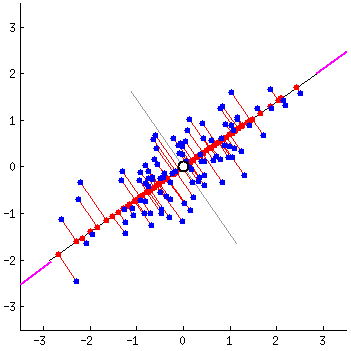
\includegraphics[width=0.3\textwidth]{img/principal-components-01.png}
        \hfill
        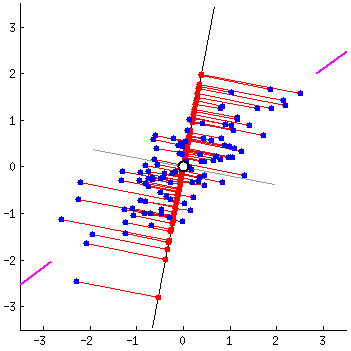
\includegraphics[width=0.3\textwidth]{img/principal-components-02.png}
        \hfill
        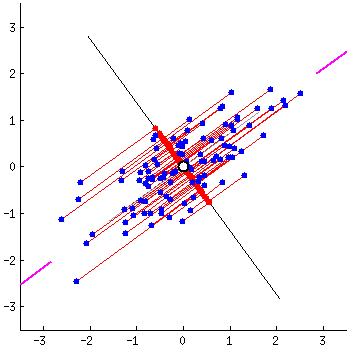
\includegraphics[width=0.3\textwidth]{img/principal-components-03.png}
        \caption{Example of PCA applied to a 2D dataset. PCs are identified as the directions that maximize the variance of the projected cloud of data. With refer to the figures, $1^{st}$ and $3^{rd}$ represent two different PCs configurations, while the $2^{nd}$ mimics the rotational transformation of the data. Credit to: \textit{Z. Jaadi}.}
    \end{figure}

    In a broad sense, the result of the PCA can be interpreted ad the `eigenvectors' of the cloud of data.

\end{frame}



\begin{frame}{Singular Value Decomposition (SVD) in the PCA approach}

    The Singular Value Decomposition (SVD) is a mathematical technique used to compute the rotational transformation needed to project the data onto the principal components.

    By definition, SVD of a matrix $\mathbf{A}_{(n \times m)}$ is defined as:

    \begin{equation}
        \mathbf{A} = \mathbf{U} \mathbf{\Sigma} \mathbf{V}^T
    \end{equation}

    Where:
    \begin{itemize}
        \item $\mathbf{U}_{(n \times n)}$ is the matrix of the left singular vectors of $\mathbf{A}$
        \item $\mathbf{\Sigma}_{(n \times m)}$ is the diagonal matrix of the singular values of $\mathbf{A}$
        \item $\mathbf{V}_{(m \times m)}$ is the matrix of the right singular vectors of $\mathbf{A}$
    \end{itemize}

    \vspace{9pt}

    Finally, the original data can be projected onto the principal components directions by means of the following transformation:
    \begin{equation}
        \mathbf{\hat{A}} = \mathbf{A} \mathbf{V}
    \end{equation}

\end{frame}



\begin{frame}{Analysis of signals via PCA}

    The clear decreasing trend of the deterministic amount, suggests that only the first(s) principal component(s) are affected by environmental conditions.
    By removing them, \textbf{we can analyze the remaining components that are likely to be strictly related to the damage itself}.

    \begin{figure}
        \centering
        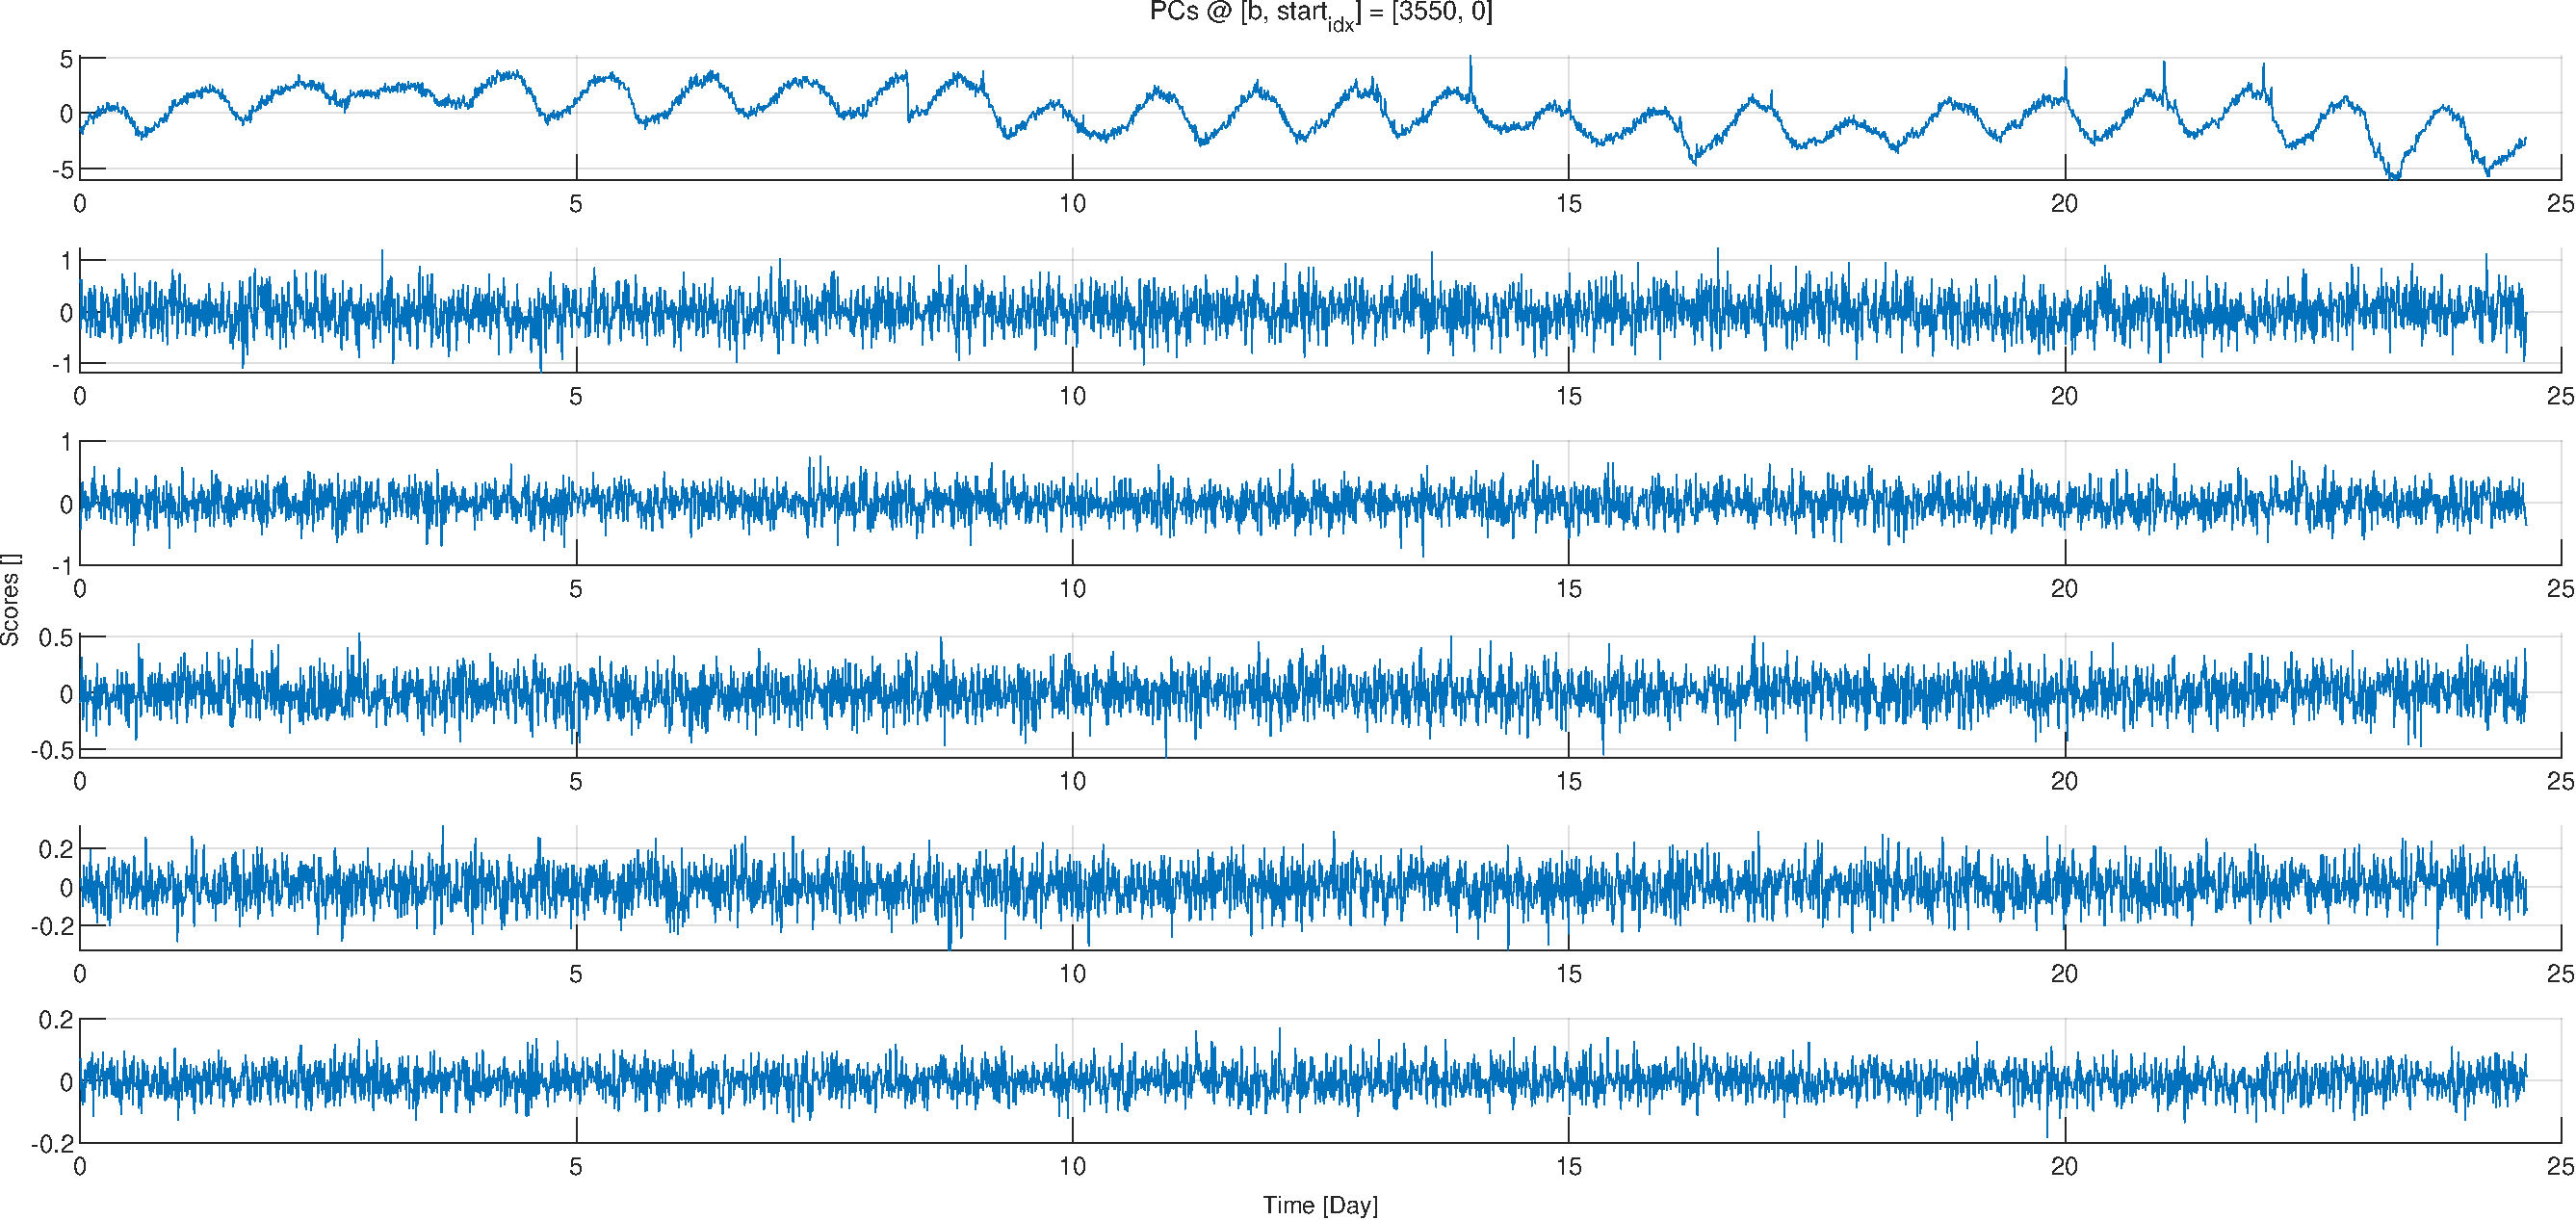
\includegraphics[width=0.9\textwidth]{img/MATLAB/PCs_01.pdf}
        \caption{Scores of the eigenfrequencies of the structure projected onto the principal components. Here, $b = 20\% \times data_{length} = 3550$.}
    \end{figure}

\end{frame}